% !TEX program = xelatex
\DocumentMetadata{lang=en} % required for transparent package
\documentclass[10pt,aspectratio=169]{beamer}
\newcommand{\subhead}[1]{\flushleft {\bf\large #1}\\}

% remove footcite numbers
\makeatletter
\def\@makefnmark{}
\makeatletter

\setbeamersize{text margin left=5mm,text margin right=5mm} 

\newcommand\focus[1]{%
	{\alert{\textbf{#1}}}
}

\usepackage{amsthm,amsmath,amssymb,braket,fontspec,unicode-math,fontenc,transparent}
\usepackage[absolute,overlay]{textpos}

\usetheme[numbering=none]{focus}
\setmathfont{latinmodern-math.otf}[range={frak,\bigcap,\bigcup}]

\usepackage[backend=bibtex,url=false,doi=false,style=authoryear]{biblatex}
\setbeamertemplate{bibliography item}{}
\bibliography{bib}
\AtBeginBibliography{\scriptsize}

\graphicspath{{./figures/}}

\setbeamerfont{title}{size=\LARGE\scshape}
\setbeamerfont{author}{size=\Large}
\setbeamerfont{institute}{size=\large}
\setbeamerfont{date}{size=\large}
\setbeamerfont{frametitle}{size=\Large\scshape}
\setbeamerfont{sectiontitle}{size=\small\scshape}
\setbeamerfont{alerted text}{series=\bfseries}

\title{Insights on Mott Transition and The Pseudogap Through the Veil of a Quantum Impurity Model}
\author{\alert{Abhirup Mukherjee}}
\date{March 19, 2025}
\institute{DPS Day '25 \\ Department of Physical Sciences, IISER Kolkata}
\titlegraphic{
	\vspace{20pt}
	\hfill
\includegraphics[width=0.1\textwidth]{epqm_logo_mod.jpeg}\hspace*{20pt}
\includegraphics[width=0.1\textwidth]{dps_logo.jpeg}\hspace*{30pt}
}

\begin{document}

\centering

\begin{frame}
\maketitle
\end{frame}

\begin{frame}{}
\hspace*{\fill}
\begin{minipage}{0.1\textwidth}
	
\includegraphics[width=\textwidth]{epqm_logo_mod.jpeg}
\end{minipage}
\begin{minipage}{0.25\textwidth}
	\centering
	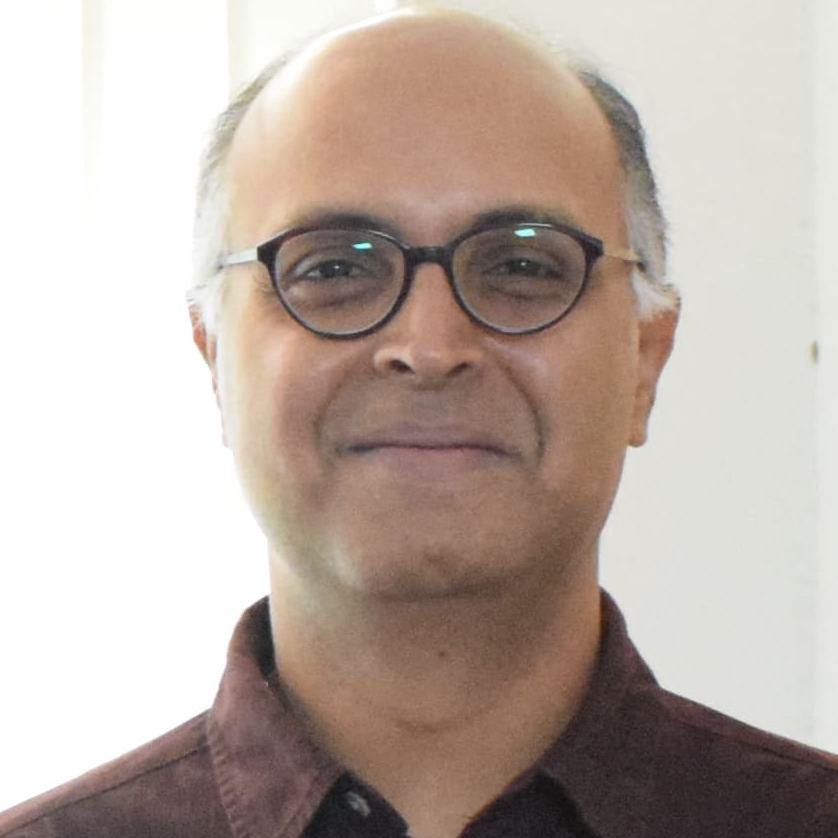
\includegraphics[width=0.6\textwidth]{slal.jpg}\\
	\footnotesize{{\bf \underline{Prof. Siddhartha Lal}}\\
	}
\end{minipage}
\begin{minipage}{0.25\textwidth}
	\centering
	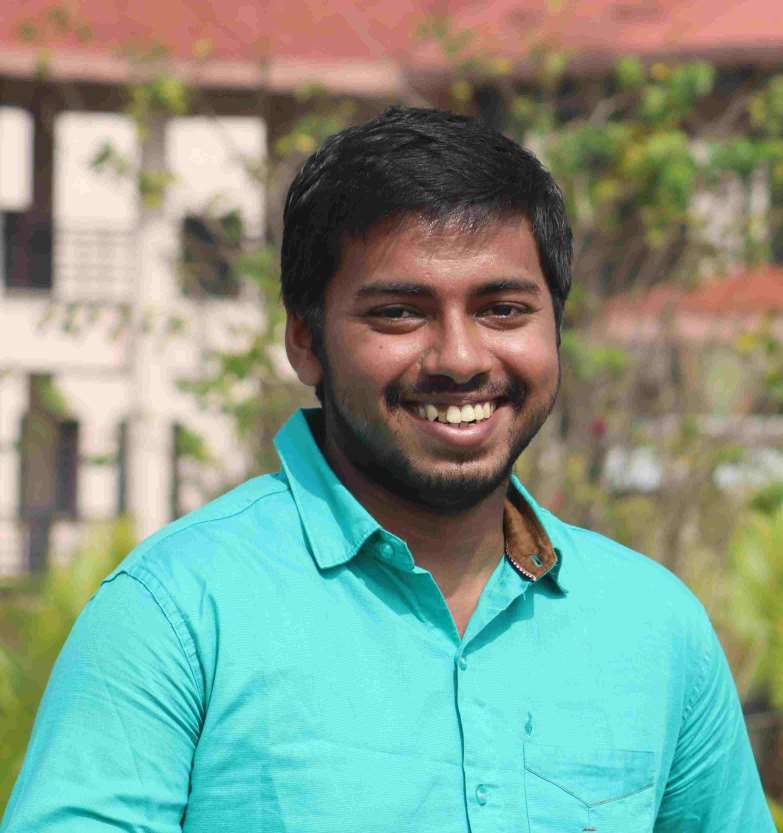
\includegraphics[width=0.6\textwidth]{debraj.png}\\
	\footnotesize{{\bf Debraj Debata}\\
	}
\end{minipage}
\begin{minipage}{0.25\textwidth}
	\centering
	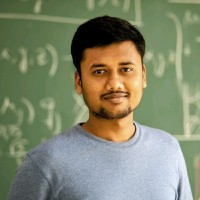
\includegraphics[width=0.6\textwidth]{spatra.jpeg}\\
	\footnotesize{{\bf Siddhartha Patra}\\
	(Multiverse Computing)}
\end{minipage}
\begin{minipage}{0.1\textwidth}
	
\includegraphics[width=\textwidth]{dps_logo.jpeg}
\end{minipage}
\hspace*{\fill}
\\
\vspace*{\fill}
\begin{minipage}{0.12\textwidth}

\includegraphics[width=\textwidth]{IISER-K_Logo.png}
\end{minipage}
\hspace*{\fill}
\begin{minipage}{0.69\textwidth}
\centering
\alert{$\sim\sim\sim\sim\sim\sim\sim\sim\sim\sim\sim\sim\sim\sim\sim$ }\\
\alert{Financial support by IISER K and SERB is gratefully acknowledged.}\\
\alert{$\sim\sim\sim\sim\sim\sim\sim\sim\sim\sim\sim\sim\sim\sim\sim$ }\\
\end{minipage}
\hspace*{\fill}
\begin{minipage}{0.12\textwidth}

\includegraphics[width=\textwidth]{SERB.png}
\end{minipage}
\vspace*{\fill}

\hspace*{\fill}
\begin{minipage}{0.3\textwidth}
	\centering
	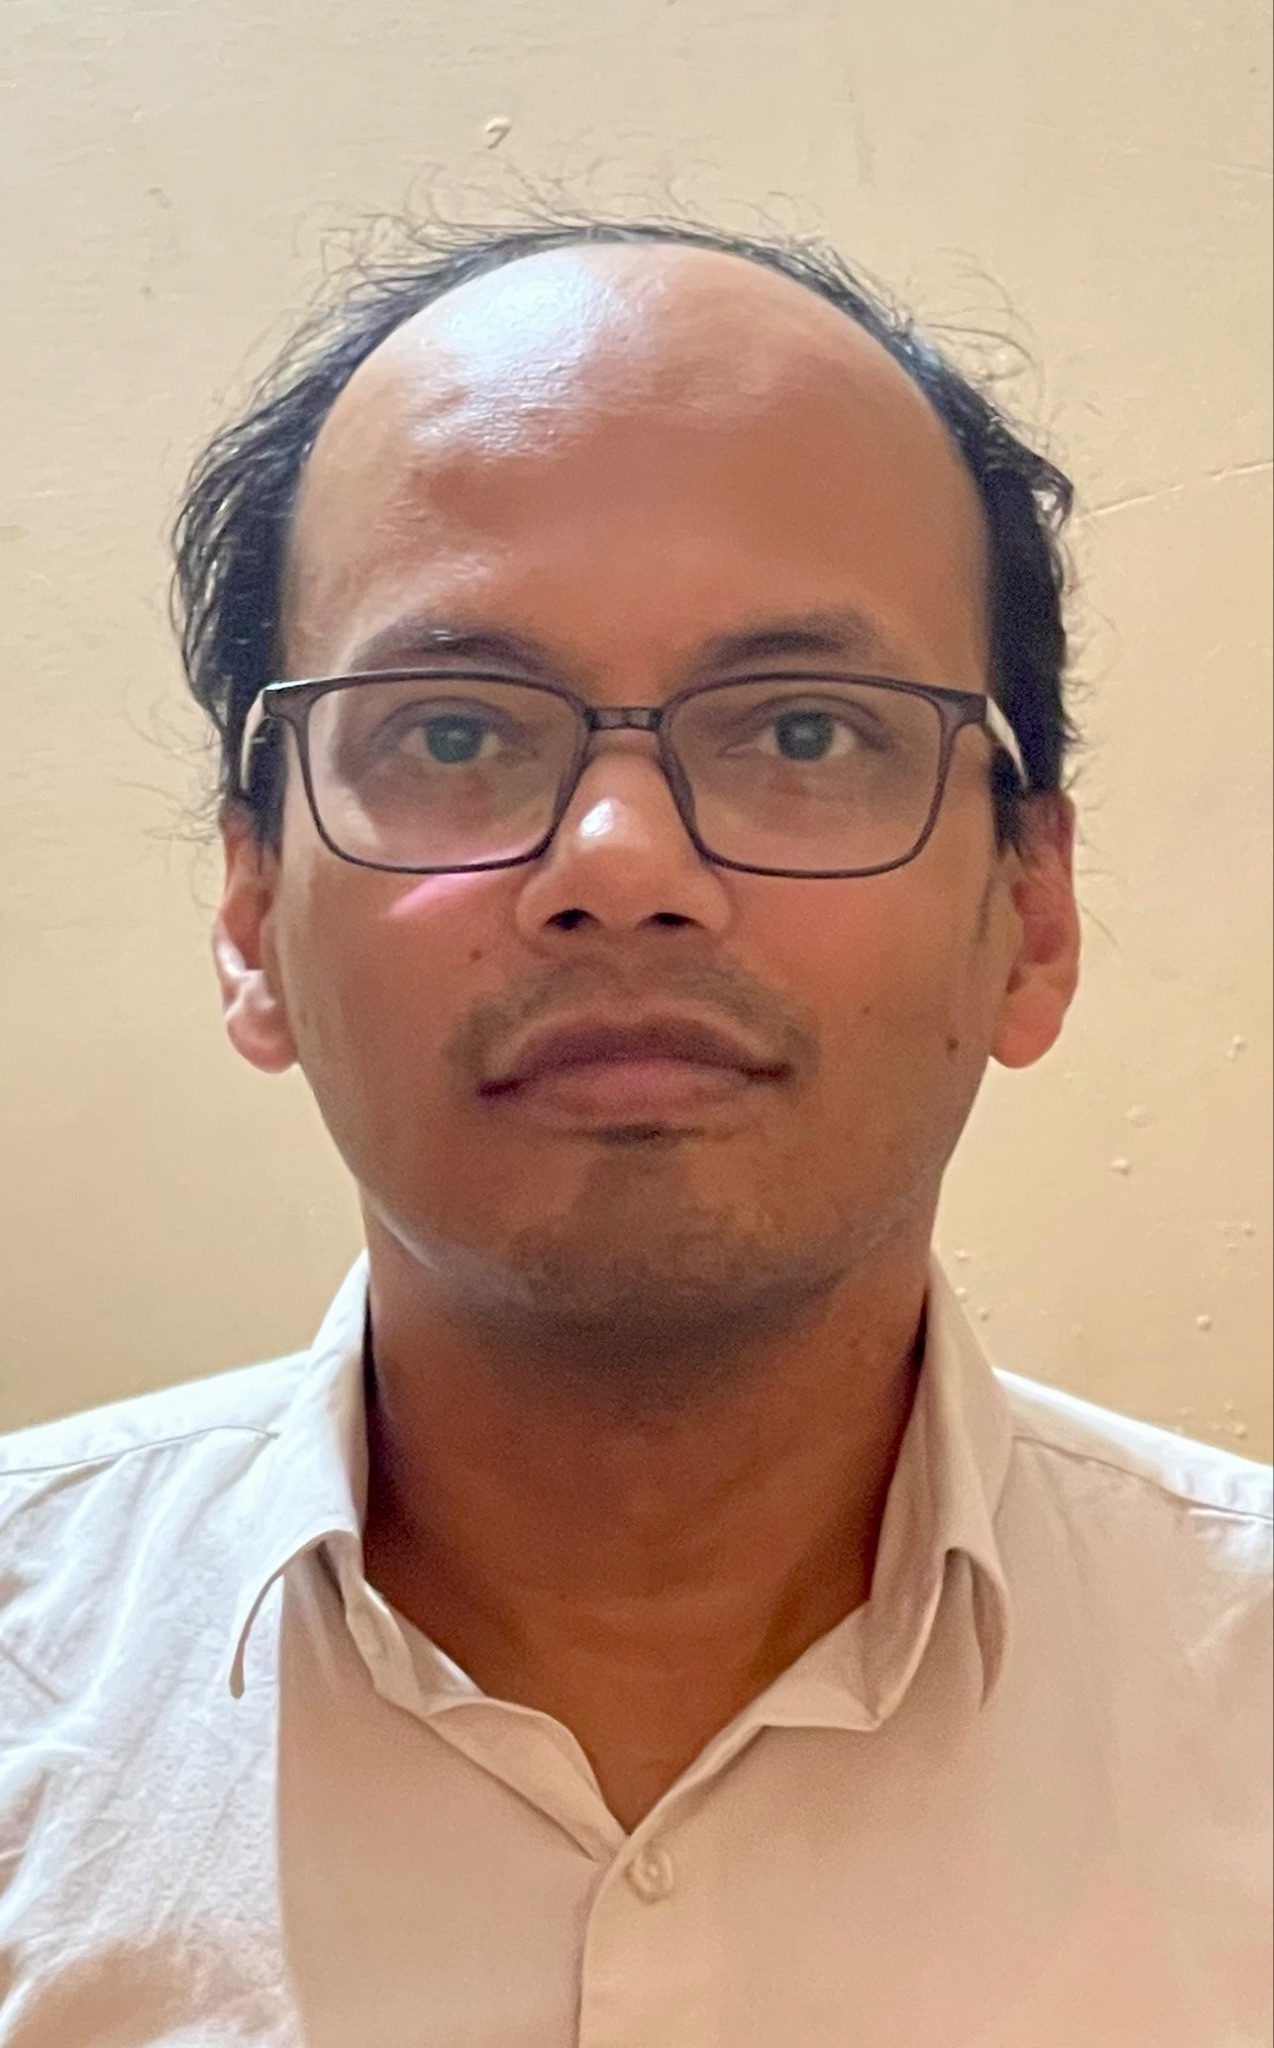
\includegraphics[width=0.35\textwidth]{anamitra.jpg}\\
	\footnotesize{{\bf Prof. Anamitra Mukherjee}\\
	(NISER Bhubaneshwar)}
\end{minipage}
\hspace*{\fill}
\begin{minipage}{0.3\textwidth}
	\centering
	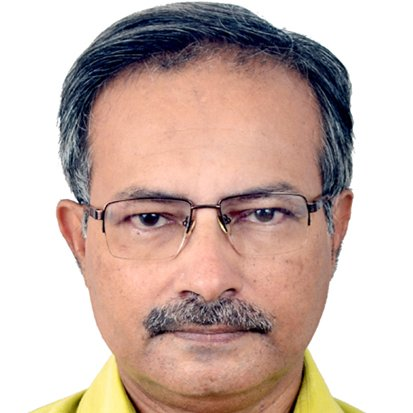
\includegraphics[width=0.45\textwidth]{arghya.jpg}\\
	\footnotesize{{\bf Prof. Arghya Taraphder}\\
	(IIT Kharagpur)}
\end{minipage}
\hspace*{\fill}
\begin{minipage}{0.3\textwidth}
	\centering
	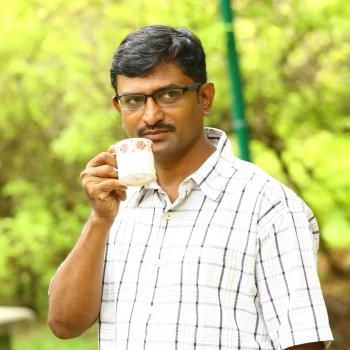
\includegraphics[width=0.45\textwidth]{nsv.jpeg}\\
	\footnotesize{{\bf Prof. N. S. Vidhyadhiraja}\\
	(JNCASR Bangalore)}
\end{minipage}
\hspace*{\fill}
\end{frame}

\begin{frame}{The Advent of Quantum Materials}
	\begin{itemize}
		\item Display exotic properties arising due to strong electronic/spin \alert{interactions}.\\
		\item \alert{Examples}: heavy fermion compounds (CePd$_2$Si$_2$), copper oxides (La$_{2−x}$Sr$_x$CuO$_4$), iron pnictides (BaFe$_2$(As$_{1−x}$P$_x$)$_2$), twisted bilayer graphene.
	\end{itemize}

	\uncover<2->{
	\subhead{What Makes Them Special - Phenomenology of The Cu-O Superconductors}
	\flushleft
	\begin{itemize}
	\uncover<3->{\item Cu-O planes separated by insulating layers that can be doped.}
	\uncover<4->{\item Strange metal phase beyond 1-particle description (\alert{breakdown of perturbation theory})}
	\uncover<5->{\item Pseudogap phase has Fermi arcs and competing fluctuations (\alert{strong correlations})}
	\uncover<6->{\item Superconductivity is \alert{unconventional} (gap vanishes at points on Fermi surface)}
	\end{itemize}

	\uncover<3->{
		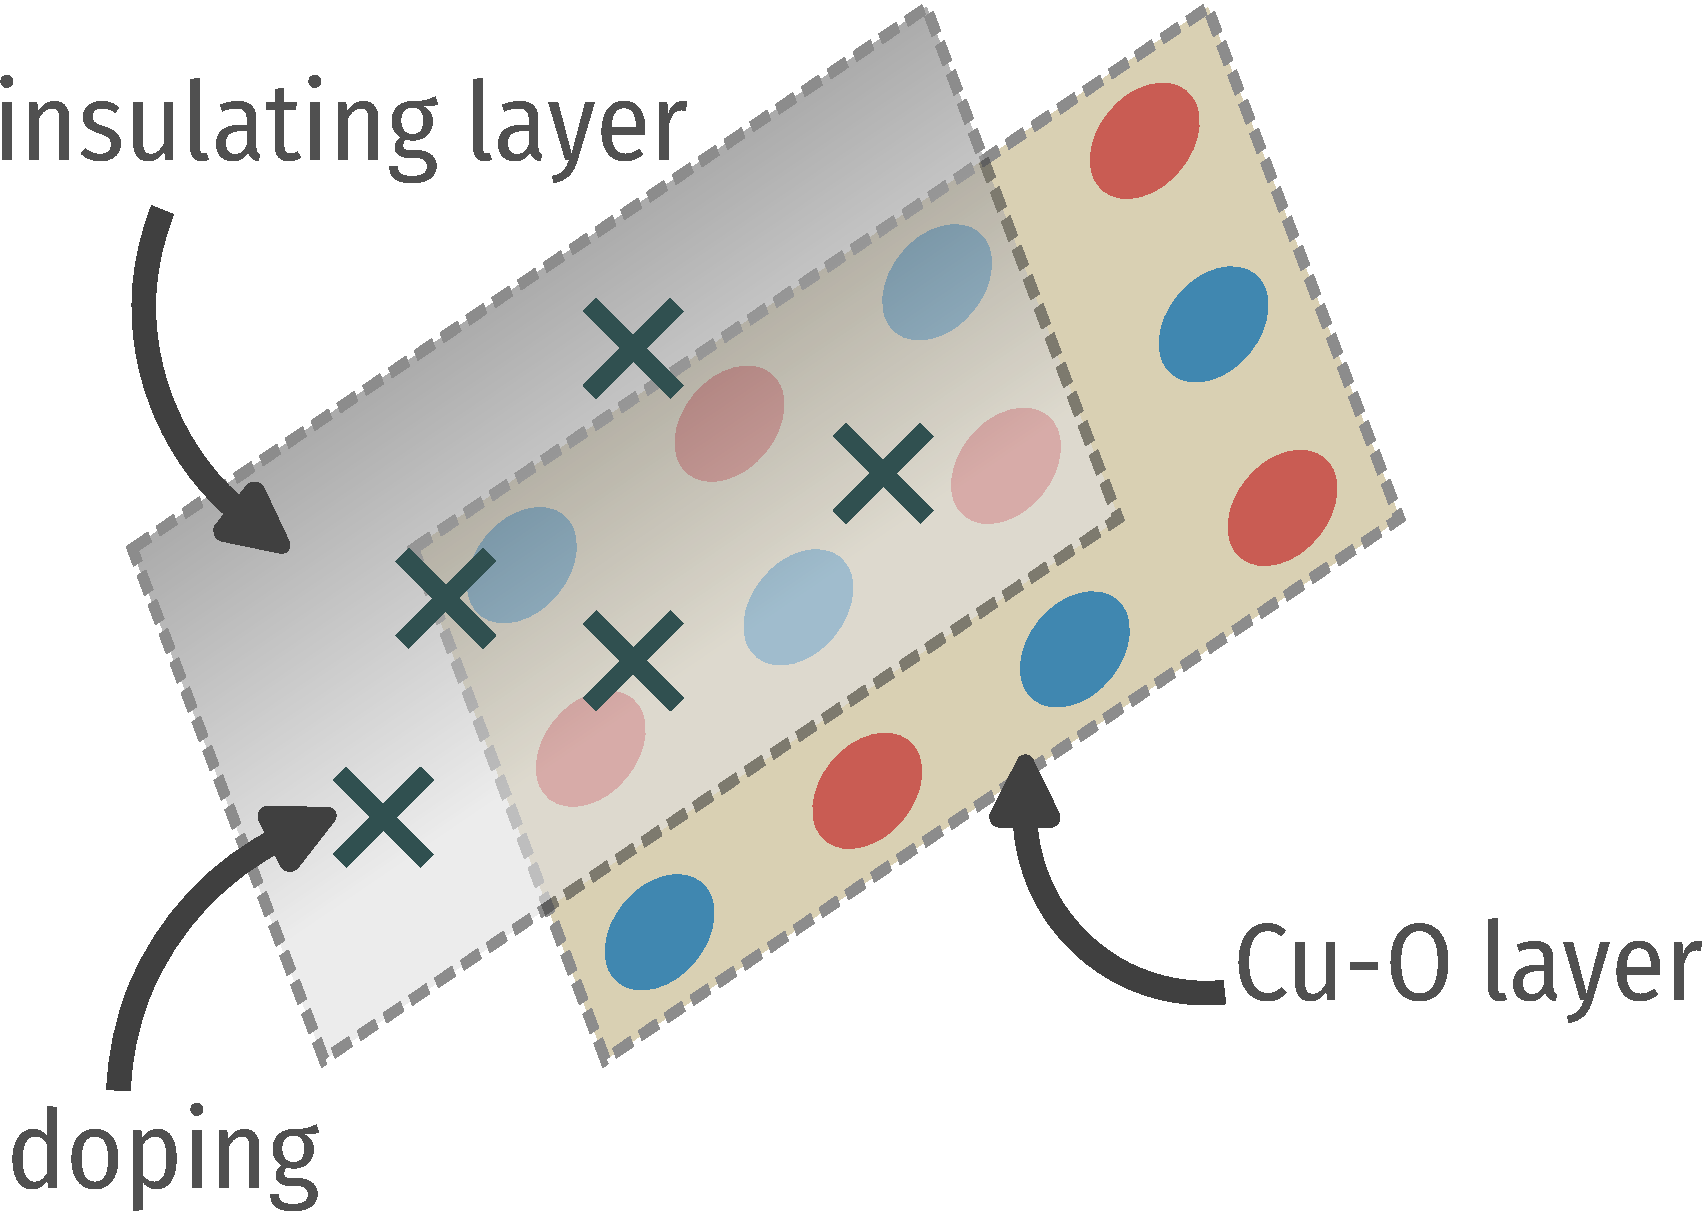
\includegraphics[width=0.3\textwidth]{cuprateStructure.pdf}
	}
	\only<4>{
		\centering
		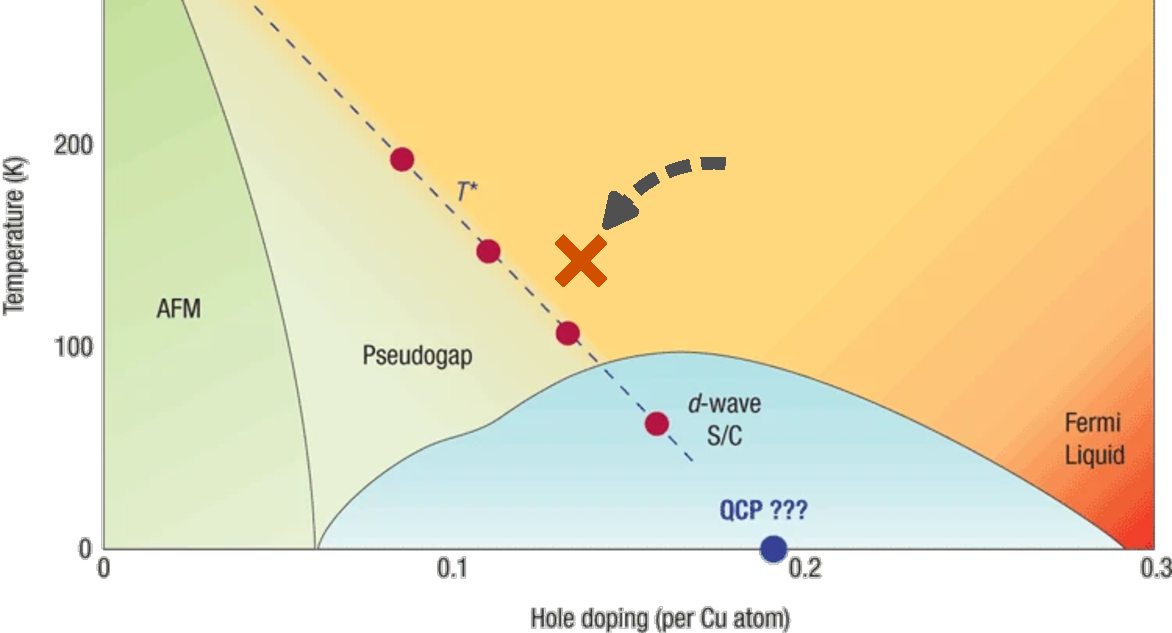
\includegraphics[width=0.3\textwidth]{cupratesNFL.pdf}
		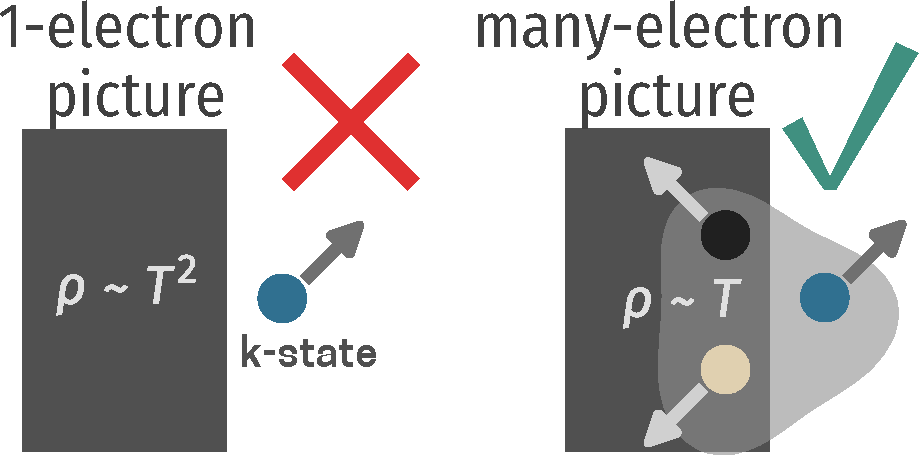
\includegraphics[width=0.35\textwidth]{NFL.pdf}
	}
	\only<5>{
		\centering
		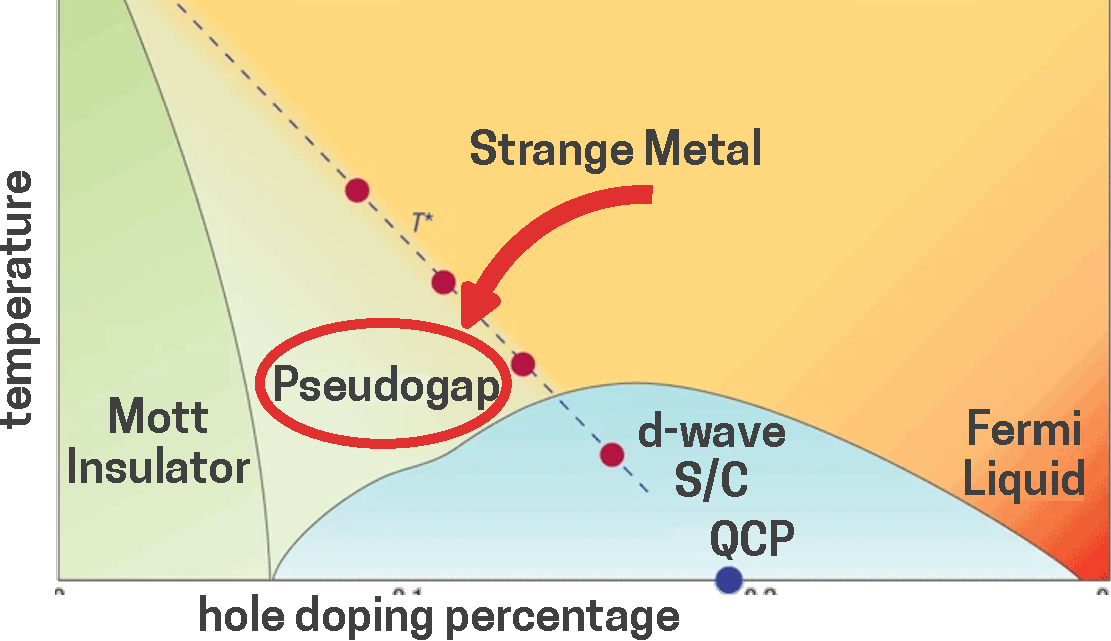
\includegraphics[width=0.3\textwidth]{cupratesPG.pdf}
		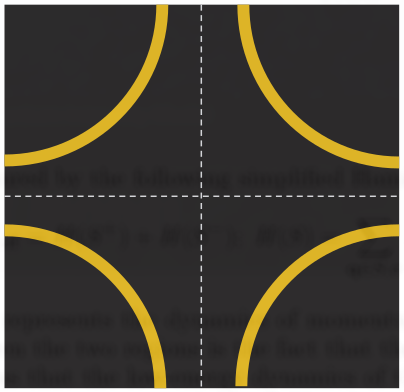
\includegraphics[width=0.17\textwidth]{fermiArc0.png}
		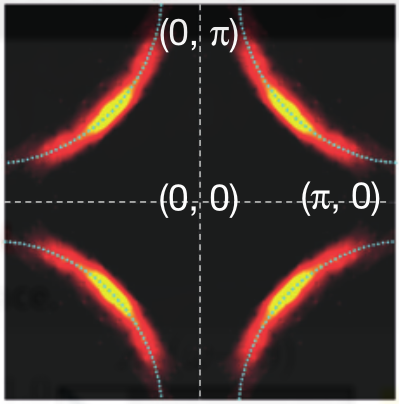
\includegraphics[width=0.17\textwidth]{fermiArc1.png}
	}
	\only<6>{
		\centering
		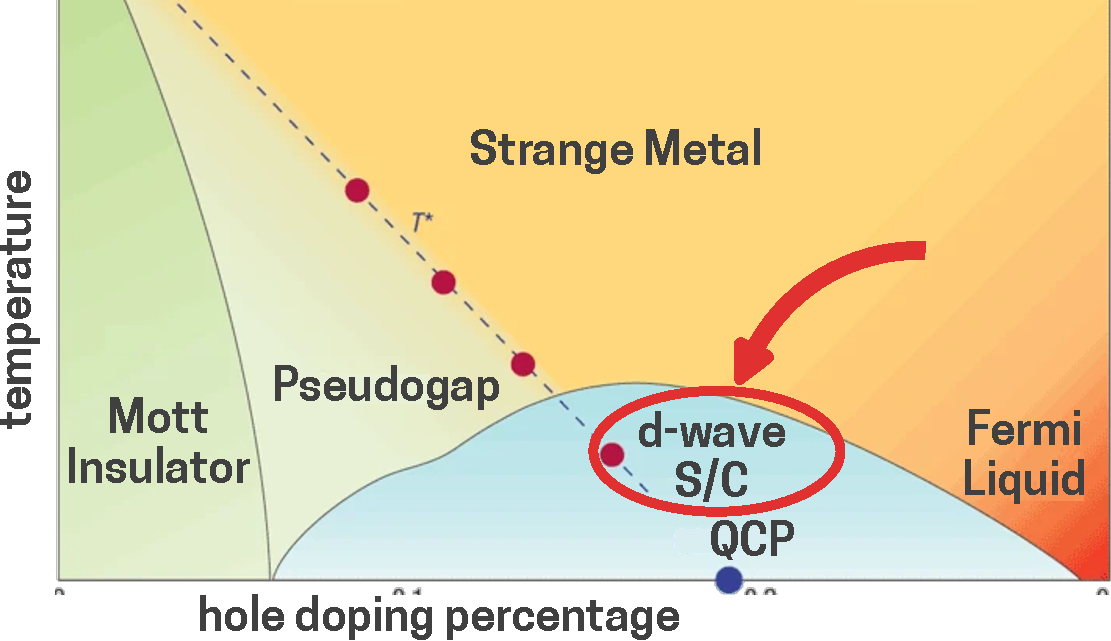
\includegraphics[width=0.3\textwidth]{cupratesSC.pdf}
		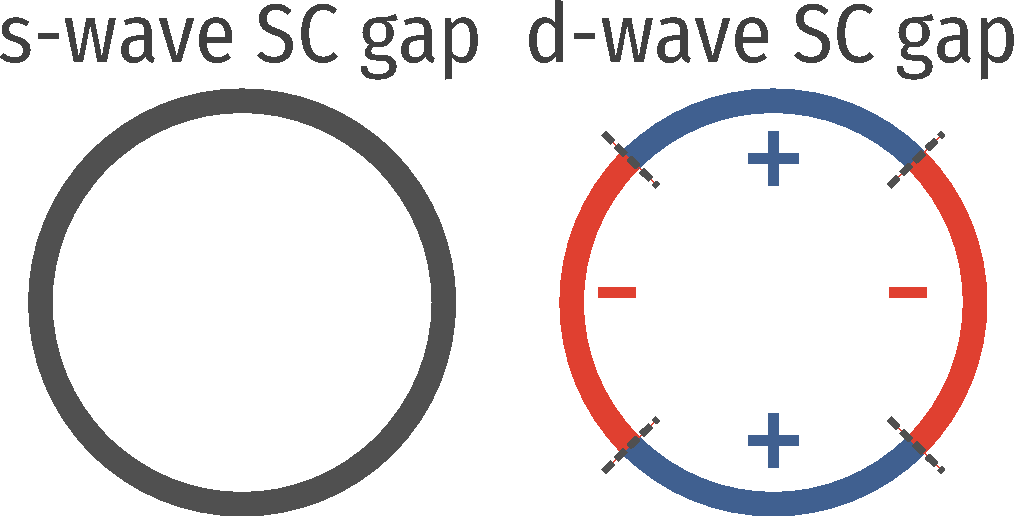
\includegraphics[width=0.35\textwidth]{dwave.pdf}
	}
	}
\end{frame}

\begin{frame}{Open Questions}
	\uncover<1->{
	\begin{minipage}{0.65\textwidth}
	The ``normal phases" remain \alert{ill-understood}:
	\begin{itemize}
		\item simple and universal mechanism for strange metals (akin to Fermi liquid theory)
		\item Microscopic understanding of the pseudogap phase
		\item How to connect \(T=0\) results to those at \(T > 0\)?
	\end{itemize}
	\end{minipage}
	\begin{minipage}{0.34\textwidth}
	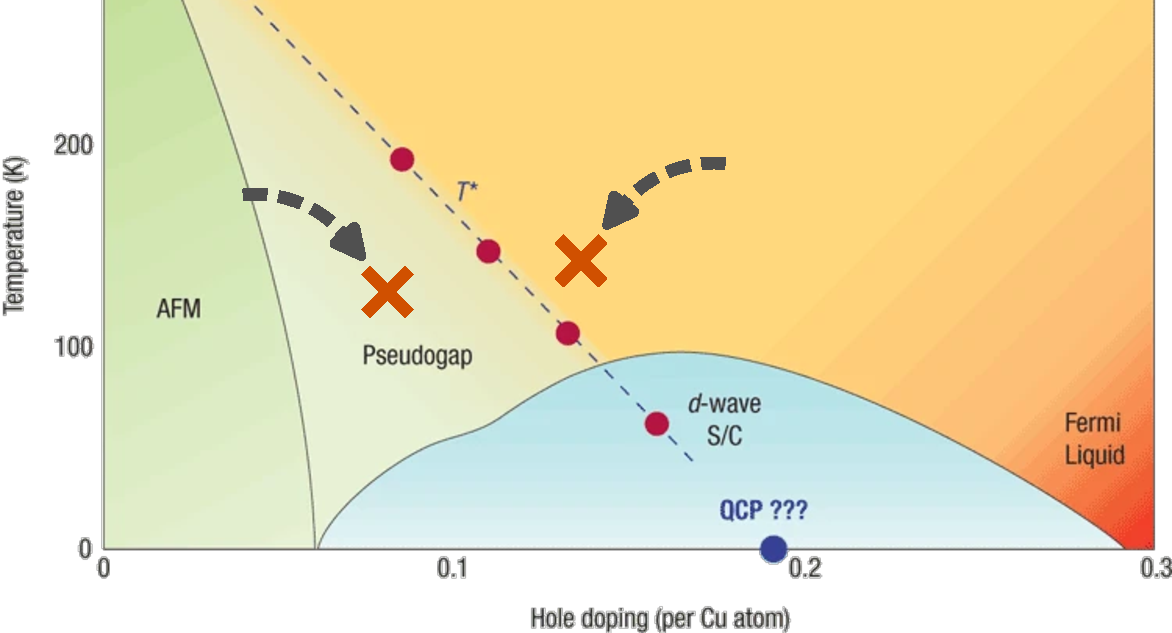
\includegraphics[width=\textwidth]{cupratesNFLPG.pdf}\\
	\end{minipage}
	% \vspace*{10pt}
	}
	\uncover<2->{
	\begin{minipage}{0.6\textwidth}
	Simplest model for realising these phases \\
	- the 2D \alert{Hubbard model} on square lattice
	\[ H = -t \sum_{\left<i,j \right>,\sigma}\left(c^\dagger_{i,\sigma}c_{j,\sigma} + \text{h.c.}\right) + U \sum_i n_{i \uparrow} n_{i \downarrow}\]
	\end{minipage}
	\hfill
	\begin{minipage}{0.35\textwidth}
		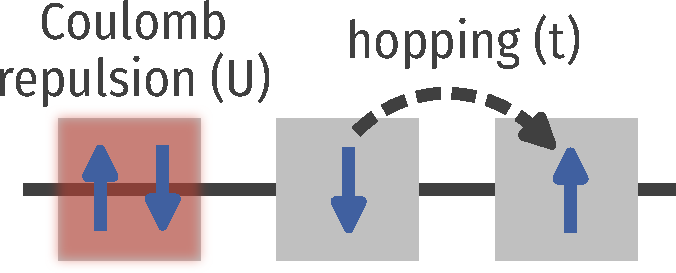
\includegraphics[width=\textwidth]{hubbard.pdf}
	\end{minipage}
	% \vspace*{10pt}
	}
	\uncover<3->{
		\flushleft
		\alert{Existing methods} suffer from a variety of problems:
		\begin{itemize}
			\item Quantum Monte Carlo suffers from fermion \alert{sign problem} at low temperatures
			\item Dynamical mean-field theory: low lack of \alert{\(k-\)space resolution} \& large computation cost
			\item DMRG only works in \alert{quasi-1D} systems
		\end{itemize}
	}
\end{frame}

\begin{frame}{A Bottom-Up Approach: Starting from an Impurity Model}
	\begin{minipage}{0.7\textwidth}
	\subhead{What is an Impurity Model?}
	\begin{itemize}[<+->]
		\item Single \alert{correlated site}, hybridising with conduction \alert{bath}
		\item Impurity-bath hybridisation respects \alert{\(C_4\) symmetry} of 2D square lattice (important!)
		\item (Much!) \alert{Simpler to solve} than Hubbard model, because of non-interacting conduction bath
	\end{itemize}
	\end{minipage}
	\hfill
	\begin{minipage}{0.25\textwidth}
		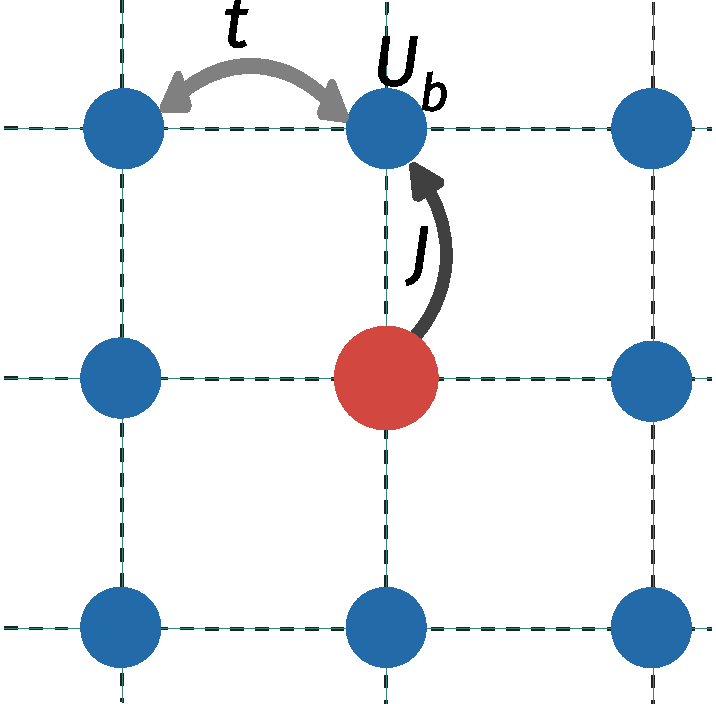
\includegraphics[width=\textwidth]{pWaveEsiam.pdf}
	\end{minipage}
	\uncover<4->{
	\begin{minipage}{0.55\textwidth}
	\subhead{Mapping to the Lattice Model}
	\begin{itemize}[<+->]
		\item Impurity model describes local environment of each site.
		\item \alert{Translation} operator maps impurity model quantities to those on the lattice model
	\end{itemize}
	\end{minipage}
	\hfill
	\begin{minipage}{0.4\textwidth}
		\only<5>{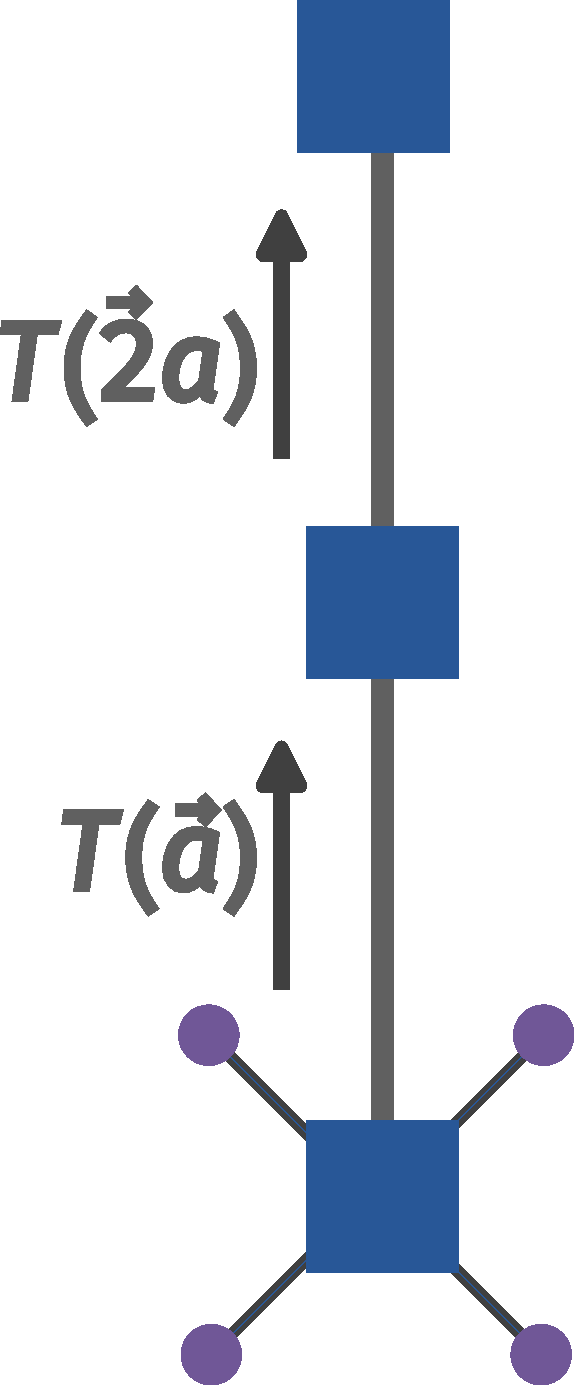
\includegraphics[width=0.3\textwidth]{translation.pdf}
		}
		\hfill
		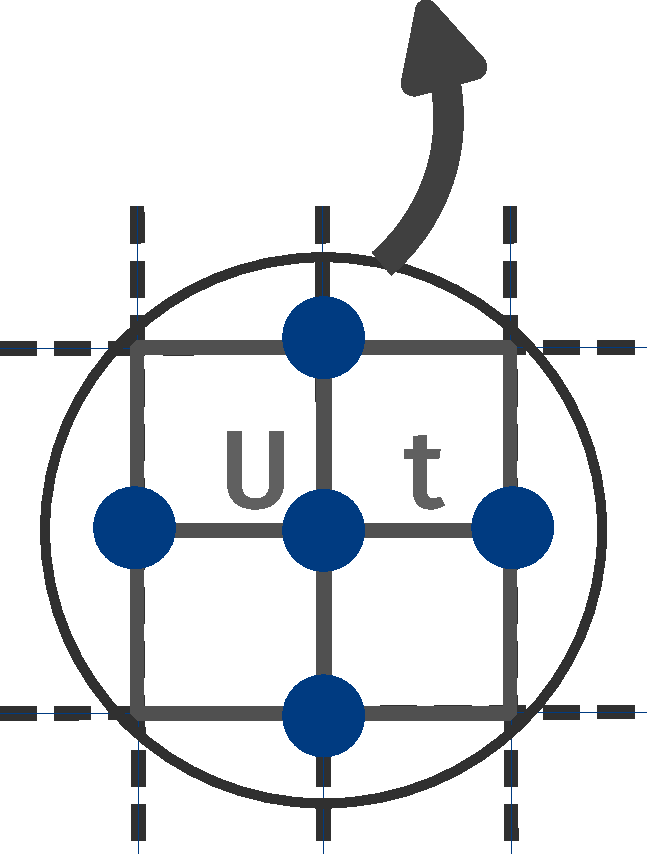
\includegraphics[width=0.5\textwidth]{tiling.pdf}
	\end{minipage}
	}
\end{frame}

\begin{frame}{Momentum-space Resolved Impurity Phase Transition}
	\begin{minipage}{0.6\textwidth}
	\alert{Raising bath correlation} \(W\) tunes the impurity model through three phases
	\uncover<2->{\begin{itemize}
		\uncover<2->{\item Impurity \alert{strongly coupled} to Fermi surface}
		\uncover<3->{\item Impurity coupled \alert{only to parts} of Fermi surface}
		\uncover<4->{\item Impurity \alert{decoupled} from the Fermi surface}
	\end{itemize}
	}
	\end{minipage}
	\uncover<1->{
	\begin{minipage}{0.35\textwidth}
	\only<2>{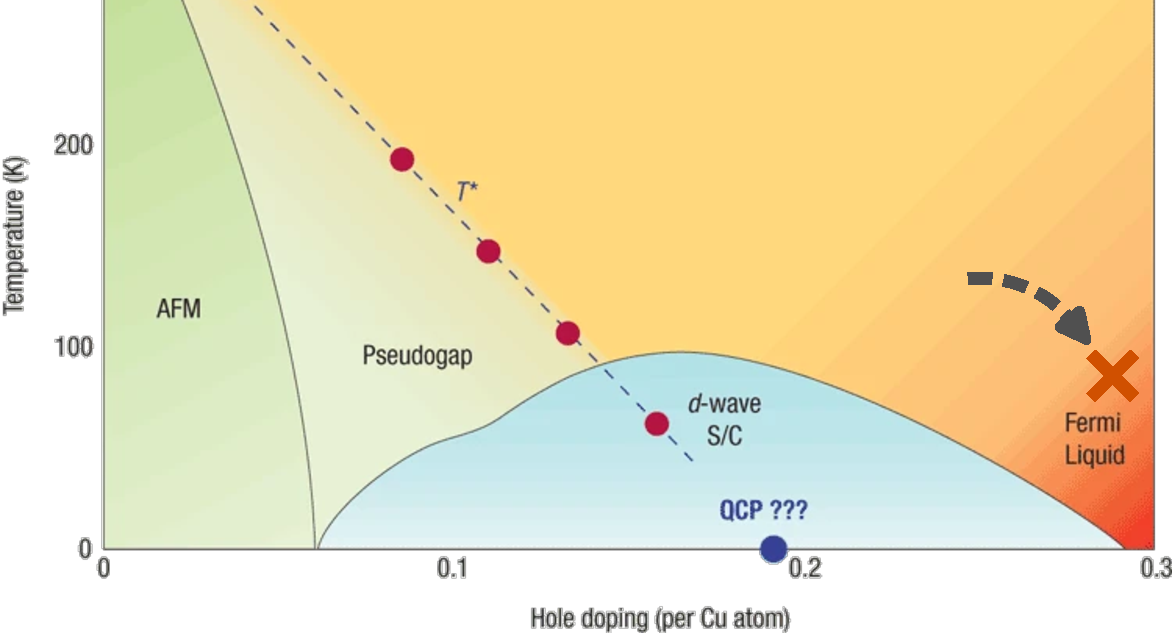
\includegraphics[width=\textwidth]{cupratesFL.pdf}}
	\only<3>{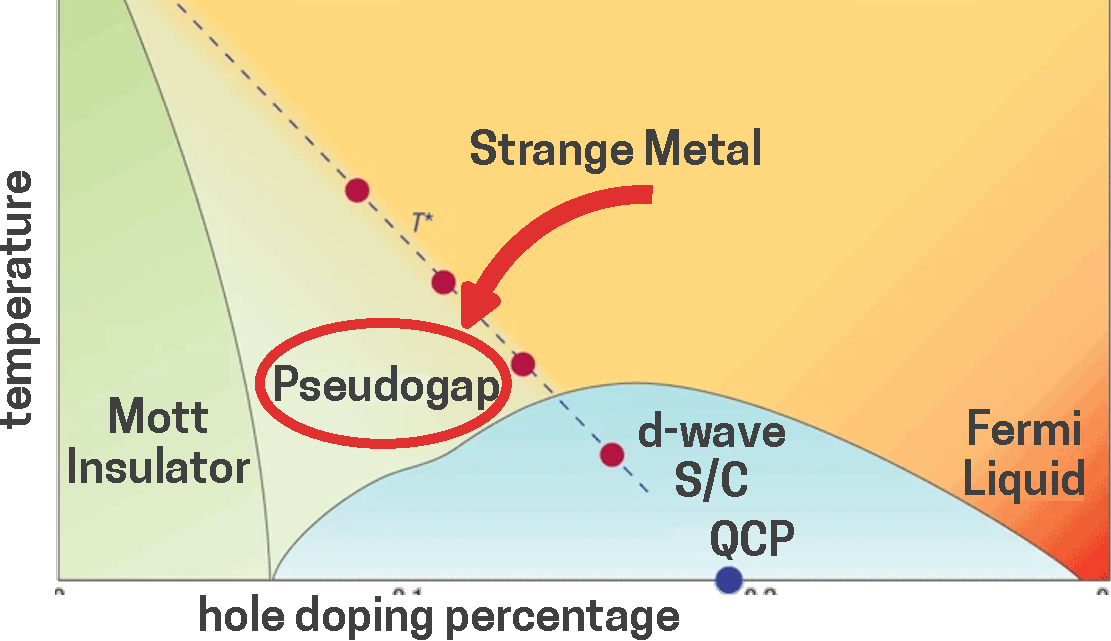
\includegraphics[width=\textwidth]{cupratesPG.pdf}}
	\only<4>{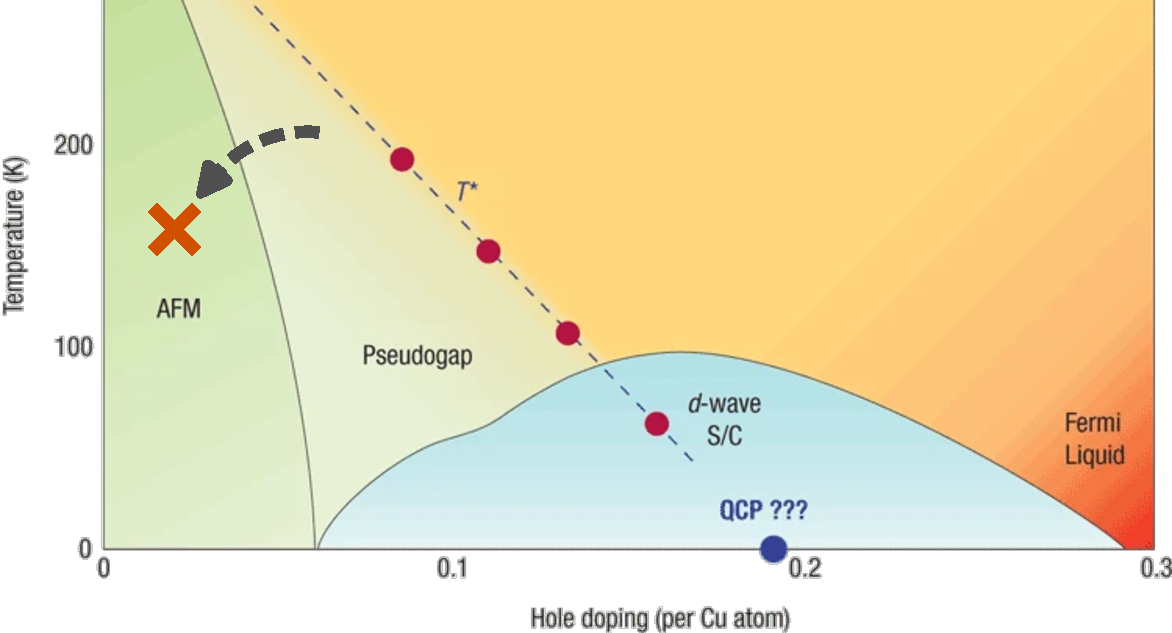
\includegraphics[width=\textwidth]{cupratesMI.pdf}}
	\end{minipage}
	}

	\uncover<1->{
	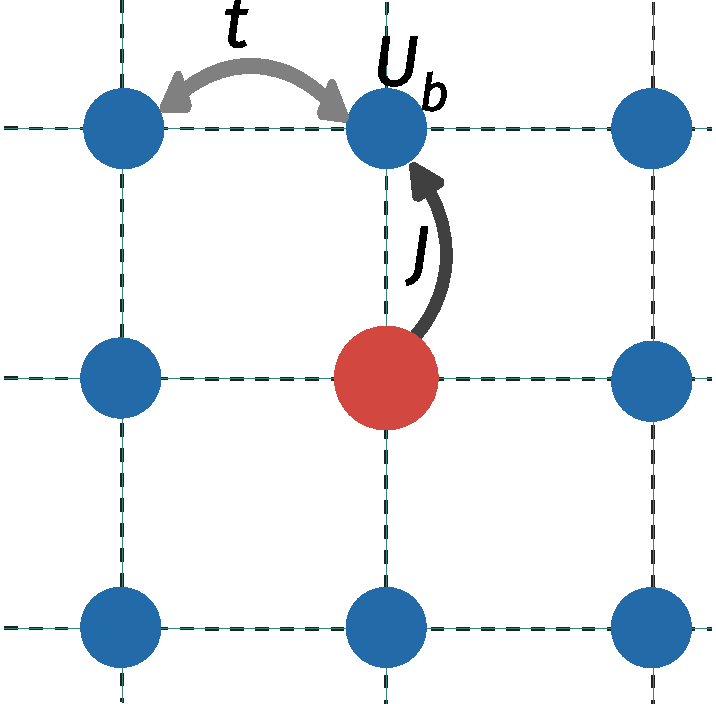
\includegraphics[width=0.2\textwidth]{pWaveEsiam.pdf}
	\hspace*{\fill}
	\only<2>{
		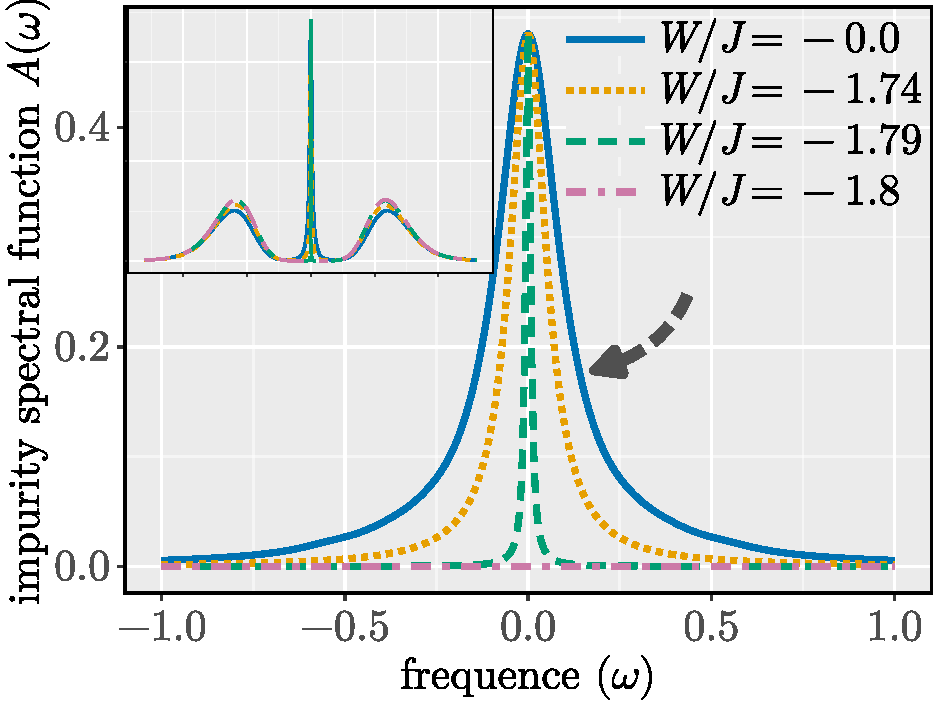
\includegraphics[width=0.35\textwidth]{localSpecFunc1.pdf}
		\hspace*{\fill}
		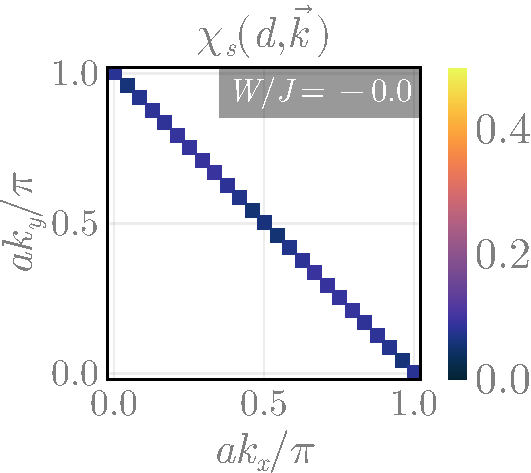
\includegraphics[width=0.3\textwidth]{SF-1.pdf}
	}
	\only<3>{
		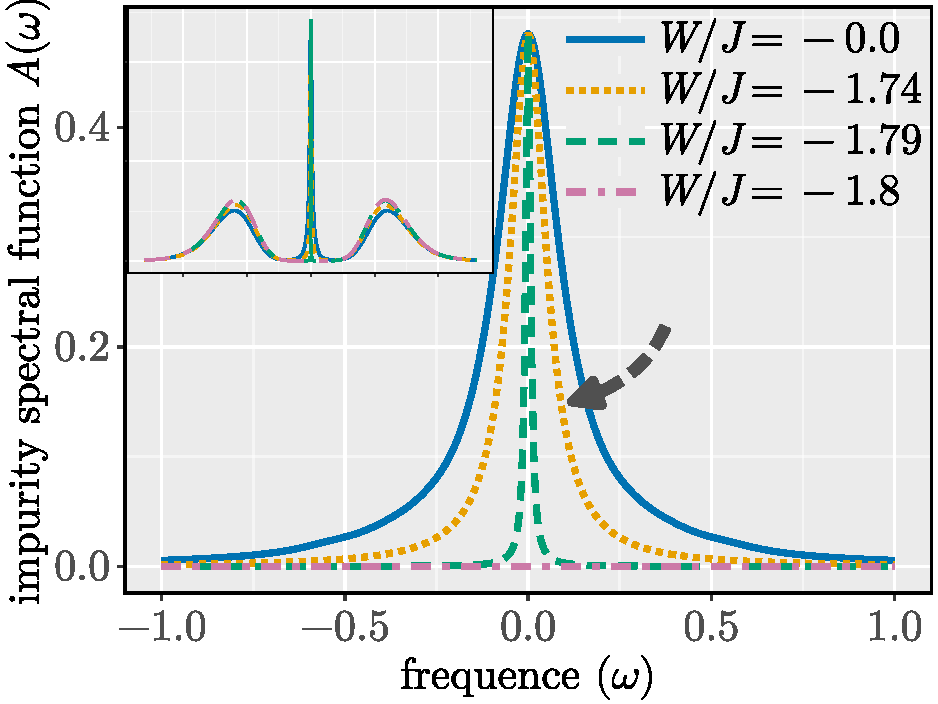
\includegraphics[width=0.35\textwidth]{localSpecFunc2.pdf}
		\hspace*{\fill}
		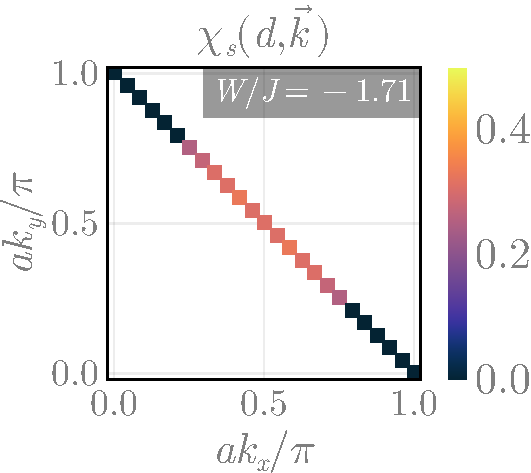
\includegraphics[width=0.3\textwidth]{SF-4.pdf}
	}
	\only<4>{
		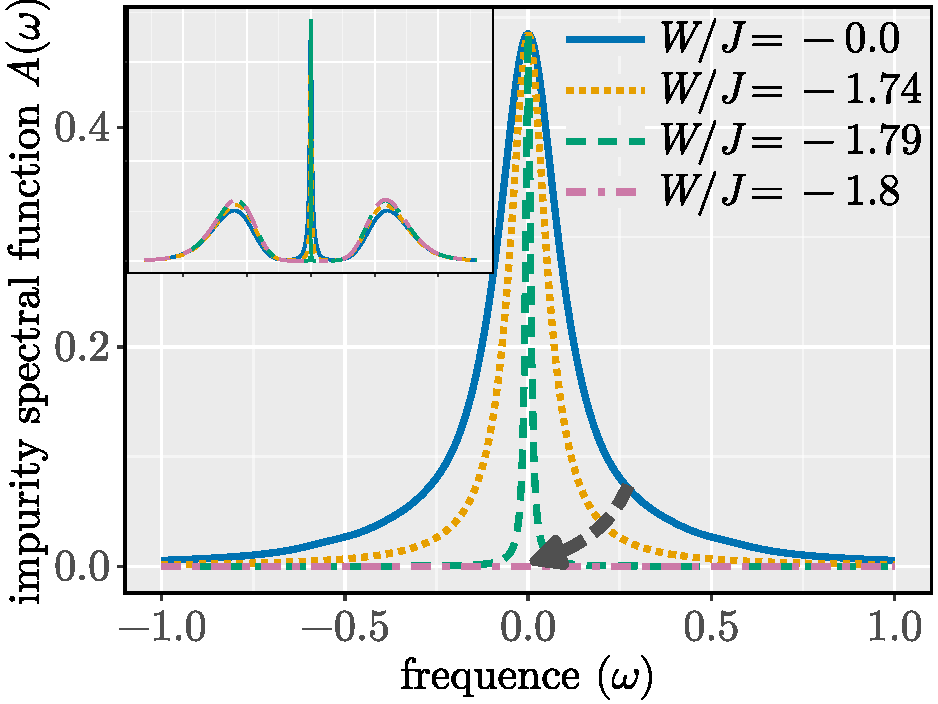
\includegraphics[width=0.35\textwidth]{localSpecFunc3.pdf}
		\hspace*{\fill}
		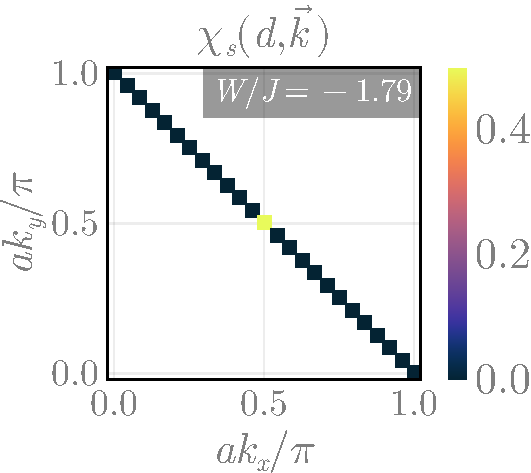
\includegraphics[width=0.3\textwidth]{SF-6.pdf}
	}
	}
\end{frame}

\begin{frame}{Pseudogapping Transition on the Lattice Model}
	\begin{minipage}{0.7\textwidth}
	\begin{itemize}
		\item Map Greens functions from impurity model to \alert{lattice model}.
		\item Momentum-space DOS reveals \alert{partially gapped} Fermi surface.
	\end{itemize}
	\end{minipage}
	\begin{minipage}{0.25\textwidth}
		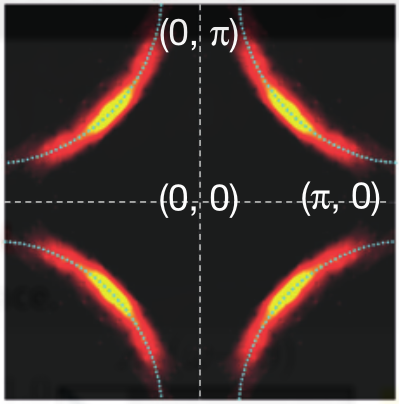
\includegraphics[width=\textwidth]{fermiArc1.png}
	\end{minipage}
	
	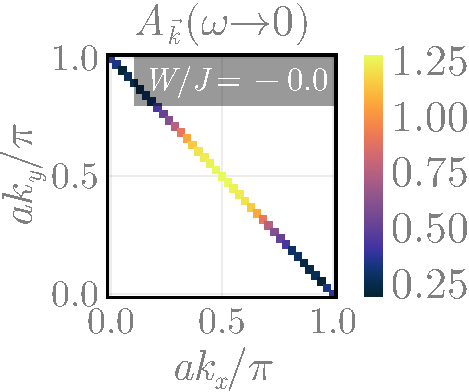
\includegraphics[width=0.31\textwidth]{kspaceDOS-1.pdf}
	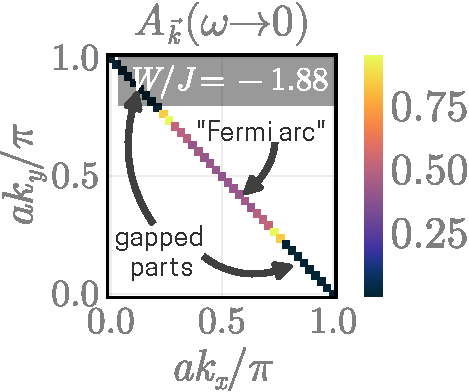
\includegraphics[width=0.31\textwidth]{kspaceDOS-3.pdf}
	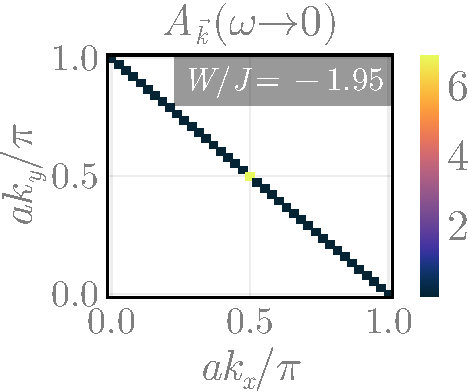
\includegraphics[width=0.31\textwidth]{kspaceDOS-4.pdf}
\end{frame}

\begin{frame}{Main takeaways}
	\uncover<1->{\begin{minipage}{0.45\textwidth}
			\alert{Simplifies} the study of lattice models through appropriate \alert{impurity models}.\\

			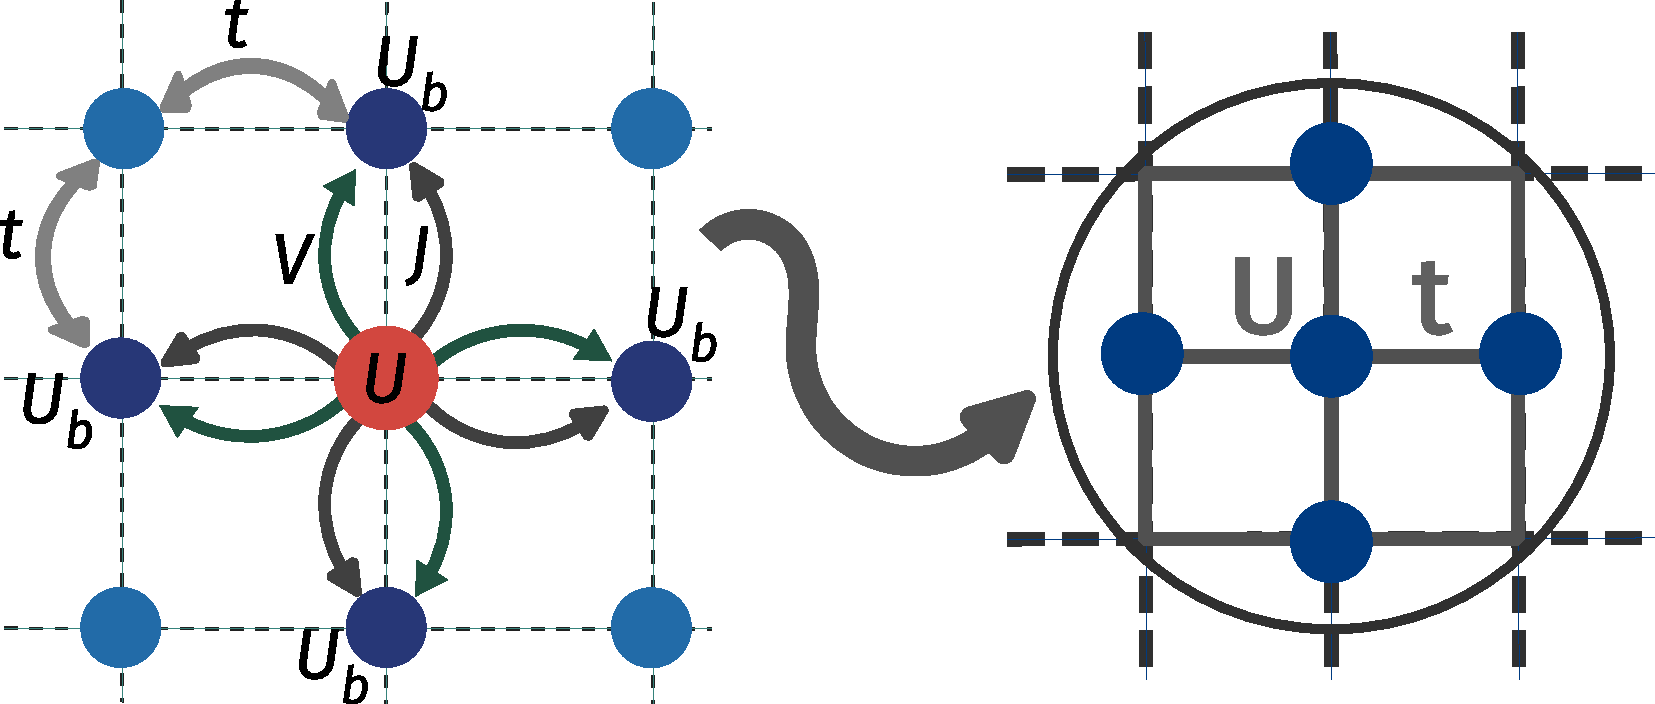
\includegraphics[height=0.4\textwidth]{tilingKey.pdf}
	\end{minipage}
	}
	\hfill
	\uncover<2->{\begin{minipage}{0.45\textwidth}
			Our impurity model realises a \alert{pseudogapping transition} in a correlated model.\\

			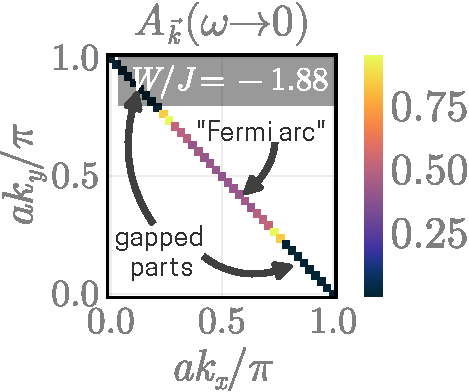
\includegraphics[height=0.4\textwidth]{kspaceDOS-3.pdf}
			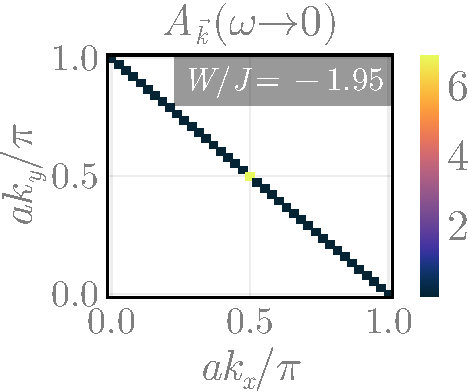
\includegraphics[height=0.4\textwidth]{kspaceDOS-4.pdf}
	\end{minipage}
	}
	\vspace*{10pt}
	\uncover<3->{
		\subhead{Generalisations and Extensions}
		\begin{itemize}[<+->]
			\item Tune impurity filling - simulate \alert{doping}!
			\item Multiple impurities - symmetry-broken or \alert{spin liquid} phases
		\end{itemize}
	}
\end{frame}

\end{document}
